%\begin{figure}[h]
%	\centering
%	\missingfigure{Sequenzdiagramm}		
%	\caption{Sequenzdiagramm - A}
%	\label{fig:sequenz-a}
%\end{figure}


%\begin{tcolorbox}
%Das dynamische Verhalten des Systems wird mittels Sequenzdiagrammen modelliert.
%Hier müssen wahrscheinlich geräteübergreifende Aufrufe modelliert werden.
%Findet dafür eine geeignete Notation und nutzt diese durchgehend! 
%Achtet weiterhin darauf, dass die anderen Methoden im Klassendiagramm zu finden sind.
%Manche Sequenzen erfordern sicherlich eine kurze schriftliche Beschreibung.
%\end{tcolorbox}

\section{Backend}

\begin{figure}[h]
	\centering
	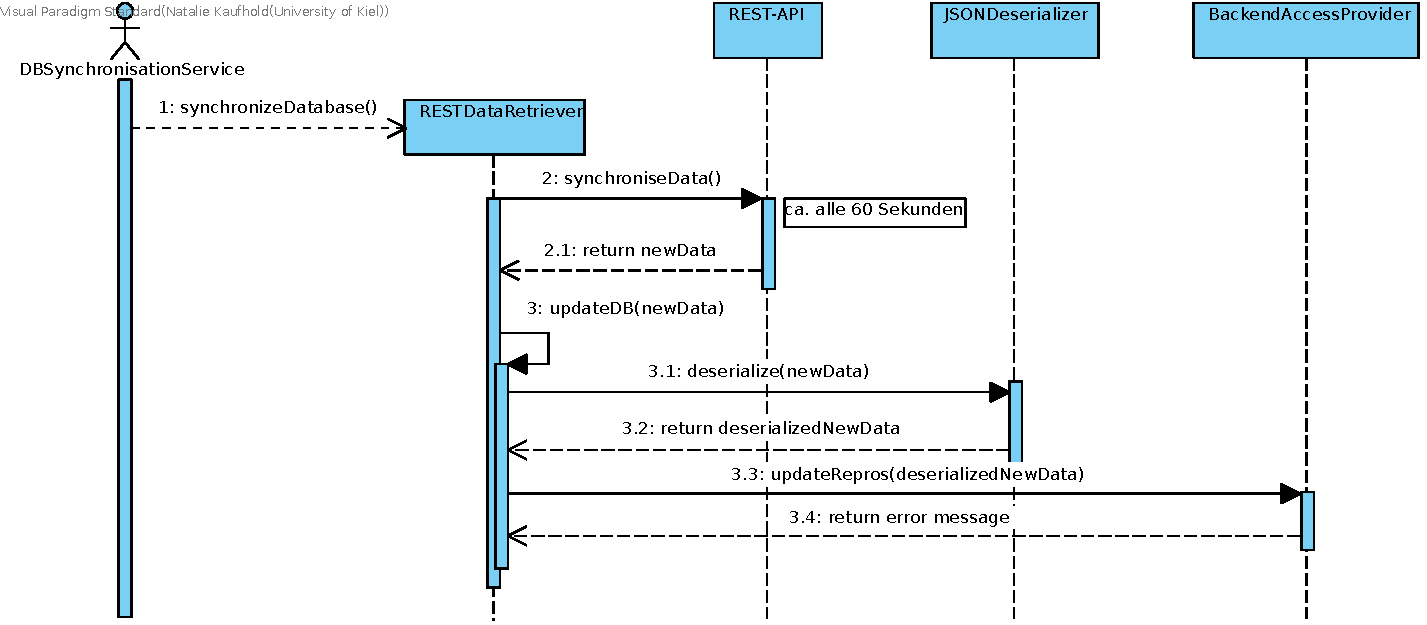
\includegraphics[width=16cm]{img/diagrams/RESThandling.pdf}	
	\caption{Sequenzdiagramm - A}
	\label{fig:sequenz-a}
\end{figure}

\noindent
Die neuen Daten werden von der REST-API als JSON zur Verfügung gestellt. Um die Daten aus der JSON-Datei in die Datenbank zu übertragen, muss  diese Datei in seine Einzelteile zerlegt werden: Dafür wird eine Instanz des JSONDeserializer genutzt, um die Daten z.B. in einen String oder eine HashMap zu konvertieren. Im nächsten Schritt werden die konvertierten Daten dann von einer Instanz des BackendAccessProviders in die Datenbank über die von Spring gestellten Repros eingetragen.
Die Klasse REST-API wird vom Kunden gestellt und verwaltet. Darauf haben wir keinen Einfluss.